% This is samplepaper.tex, a sample chapter demonstrating the
% LLNCS macro package for Springer Computer Science proceedings;
% Version 2.20 of 2017/10/04
%
\documentclass[runningheads]{llncs}
%
\usepackage{graphicx}
\usepackage{amsmath}
\usepackage{longtable}
\usepackage{float} % For precise float placement
\usepackage{subcaption} % For subtables
\usepackage{afterpage} % For forcing table to appear after current page
\usepackage{setspace} % For adjusting line spacing
\usepackage{dialogue}
% Used for displaying a sample figure. If possible, figure files should
% be included in EPS format.
%
% If you use the hyperref package, please uncomment the following line
% to display URLs in blue roman font according to Springer's eBook style:
% \renewcommand\UrlFont{\color{blue}\rmfamily}
% Used for a dialog representation

   
\begin{document}
%
\title{Conversational Task Agent}
%
%\titlerunning{Abbreviated paper title}
% If the paper title is too long for the running head, you can set
% an abbreviated paper title here
%
\author{Guilherme Fernandes\inst{1}\orcidID{60045} \and
Ricardo Silva\inst{1}\orcidID{60559} \and
Vladyslav Mikytiv\inst{1}\orcidID{60735}}
%
\authorrunning{Guilherme, Ricardo, Vladyslav}
% First names are abbreviated in the running head.
% If there are more than two authors, 'et al.' is used.
%
\institute{NOVA School Of Science and Technology}
%
\maketitle              % typeset the header of the contribution
%
\begin{abstract}
Our project focuses on creating an adaptive taskbot tailored specifically for guiding users through cooking tasks. This taskbot will utilize artificial intelligence and natural language processing to interact with users, understanding their progress and constraints in real-time. The taskbot will dynamically adjust instructions based on the ingredients and cooking tools available to the user. In instances where users encounter obstacles, such as running out of ingredients or lacking specific utensils, the taskbot will intelligently adapt the recipe, offering alternative ingredient substitutions or equipment alternatives to ensure successful completion of the dish. By providing personalised guidance our taskbot aims to enhance the culinary experience.

\keywords{Taskbot  \and Word embedding \and Natural Language Processing}
\end{abstract}
%
%
%
\section{Introduction}
In recent years, word embedding has emerged as a cornerstone technology in the field of artificial intelligence, revolutionising natural language processing (NLP) tasks. This transformative approach to representing words as dense vectors in continuous vector spaces has garnered significant attention and acclaim within the AI community. The rise of word embedding has been marked by its progression from conventional methods to the creation of sophisticated models capable of capturing intricate semantic connections among words.

The inception of word embedding can be traced back to the early 2000s when researchers began exploring methods to overcome the limitations of traditional vector space models, such as bag-of-words and one-hot encoding. These initial efforts paved the way for more advanced approaches that would later reshape the field of natural language processing (NLP).

However, it wasn't until the introduction of groundbreaking techniques like Word2Vec by Mikolov et al. in 2013 and GloVe (Global Vectors for Word Representation) by Pennington et al. in 2014 that word embedding started to gain widespread attention and adoption. These models introduced novel methodologies for learning distributed representations of words based on large corpora of text, capturing intricate semantic nuances and relationships.

The allure of word embedding lies in its ability to encode semantic meaning into dense vector representations, enabling machines to understand language in a more nuanced and contextually rich manner.

The project aims to utilize embedding algorithms and large language models to develop a dialog manager between users and the taskbot. This manager will execute user requests and guide them through processes, particularly in cooking recipes, with adaptability. Leveraging a dataset containing recipes data, including ingredients, procedural steps, and difficulty levels, we utilize OpenSearch indexing to efficiently retrieve information for user queries.


\section{Algorithms and Implementation}
\subsection{Indexing}
We must implement a search index of complex manual tasks in order to allow our system to retrieve relevant information about the tasks.

\begin{figure}[!htbp]
    \center
    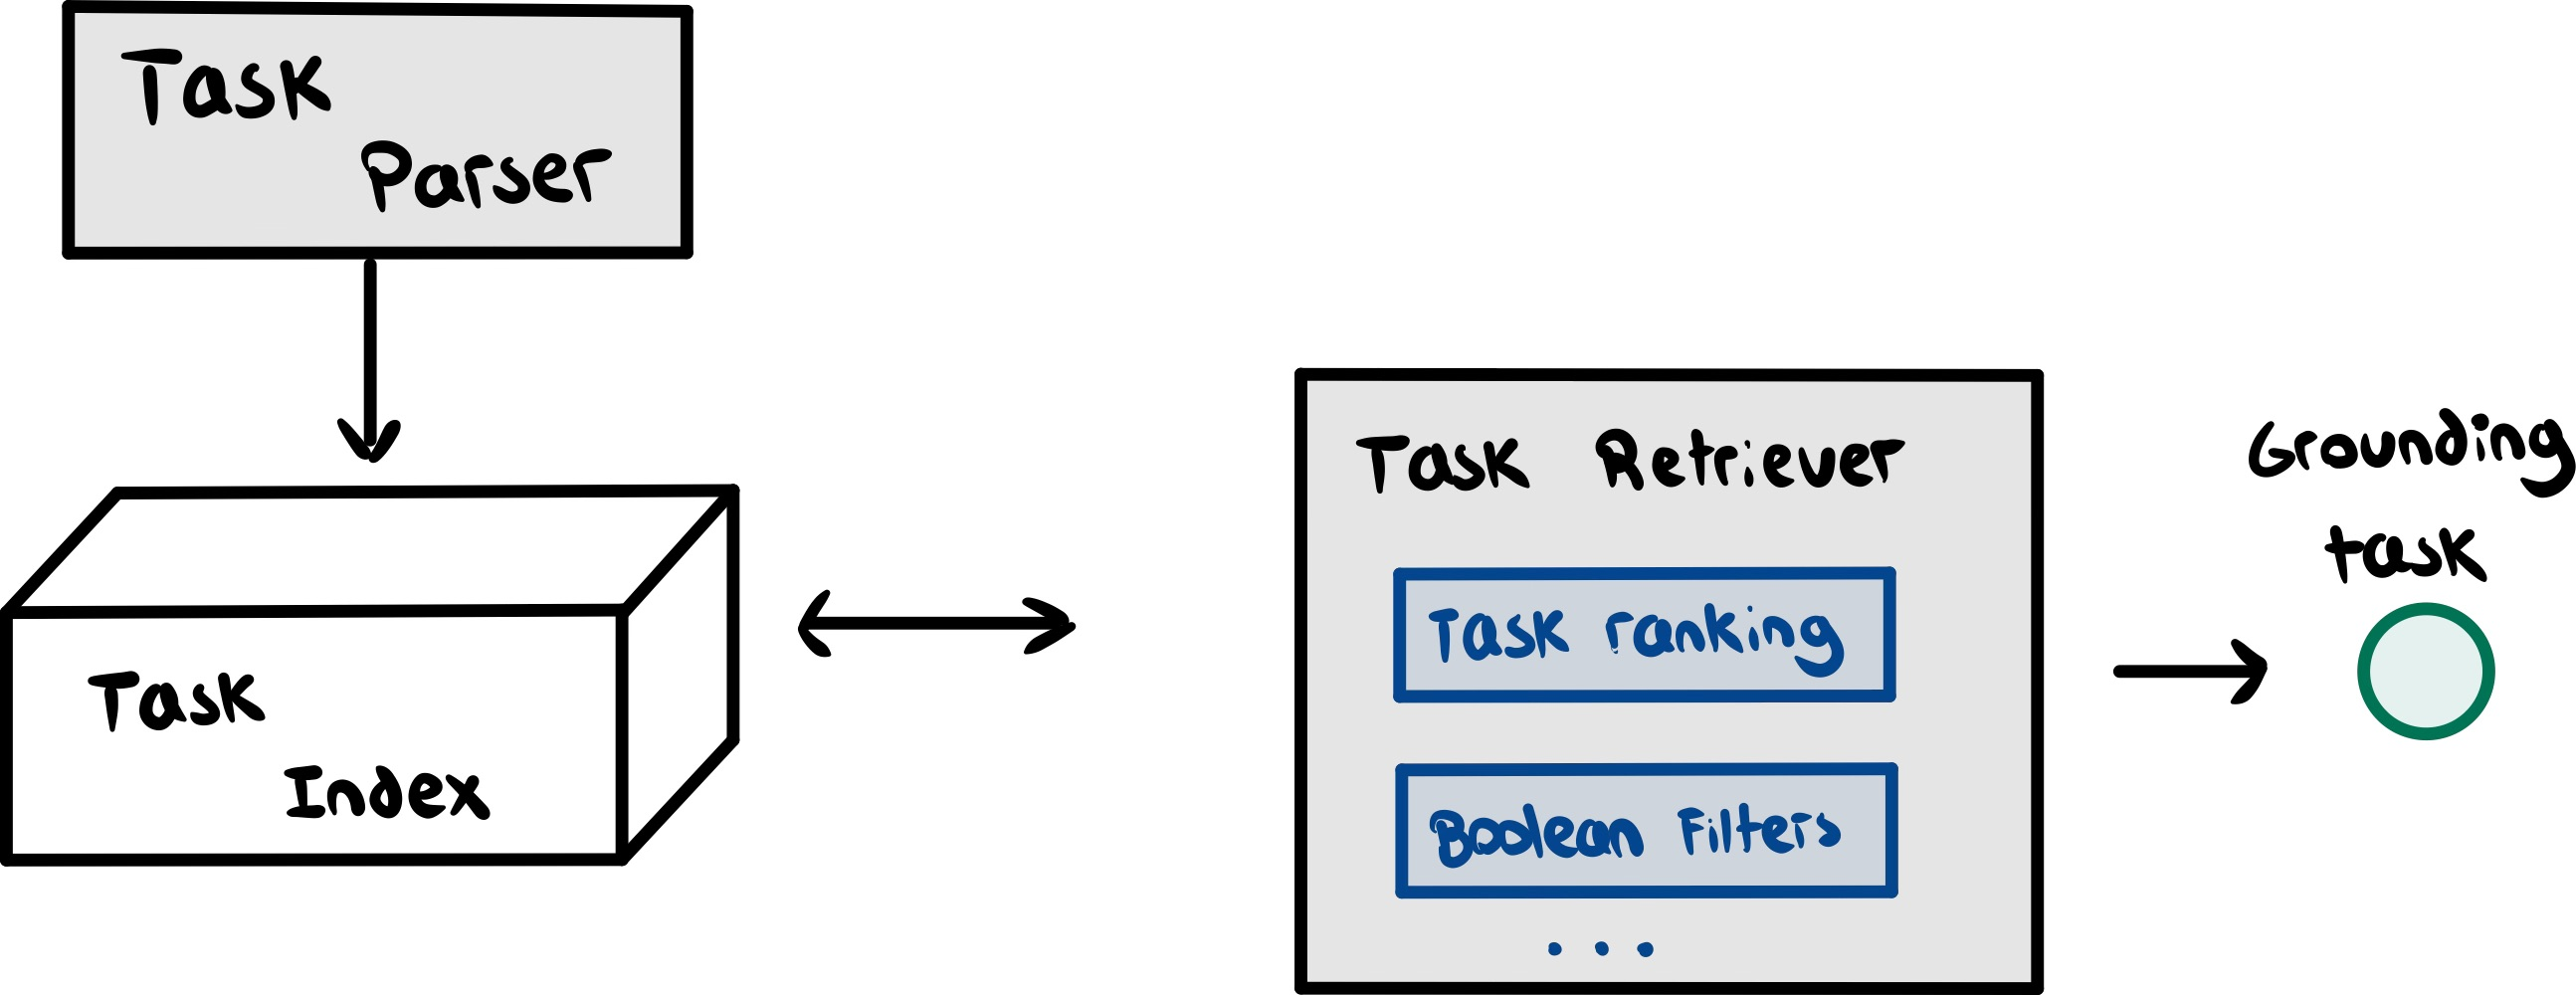
\includegraphics[scale=0.08]{images/task_retriever.jpg}
    \caption{Task retrieval}
\end{figure}

We must parse the data from the dataset which is a JSON file. We do that while we populate our indexes in OpenSearch. For each recipe we parse the JSON and send the relevant information to the index mapping that was created. We introduce a set of mappings tailored to effectively index recipe data and they are the following:

    
\begin{table}[ht]
\centering
\setlength{\abovecaptionskip}{10pt} % Adjust the spacing here
\resizebox{0.7\textwidth}{!}{%
\begin{subtable}{0.45\linewidth}
\centering
\begin{tabular}{|c|c|}
\hline
\textbf{Field} & \textbf{Data Type} \\ \hline
recipeJson & object \\ \hline
recipeName & text \\ \hline
prepTimeMinutes & integer \\ \hline
cookTimeMinutes & integer \\ \hline
totalTimeMinutes & integer \\ \hline
difficultyLevel & keyword \\ \hline
images & array of text \\ \hline
servings & float \\ \hline
\end{tabular}
\end{subtable}
\hfill % Add horizontal space between subtables
\begin{subtable}{0.45\linewidth}
\centering
\begin{tabular}{|c|c|}
\hline
\textbf{Field} & \textbf{Data Type} \\ \hline
videos & array of object \\ \hline
tools & array of text \\ \hline
cuisines & array of text \\ \hline
courses & array of text \\ \hline
diets & array of text \\ \hline
ingredients & array of object \\ \hline
stepsEmbedding & knn\_vector \\ \hline
\end{tabular}
\end{subtable}
}
\caption{Index Mapping}
\label{tab:mappings}
\end{table}

An important detail to emphasise is that our \textbf{ingredients} are a \textbf{nested type} with the properties \textbf{name} and most importantly the
corresponding \textbf{\text{ingredient\_embedding}}. We also used the mpnet-base-v2 transformer because it had better results.~\cite{mpnet}.

\subsection{Searching}
We've initiated the project by focusing on leveraging indexes for efficient dataset navigation, and OpenSearch emerges as a pivotal tool for executing queries seamlessly.

We've commenced with text-based queries, enabling users to access recipes based on various parameters such as cooking time, difficulty level, course type, or serving size.

Moreover, the integration of boolean queries adds another layer of flexibility, empowering users to refine their searches by specifying ingredients they desire or wish to avoid in their recipes.

Embedded queries stand out as particularly intriguing among our query types. By transforming user inputs into vector representations, we can uncover recipes closely related to the query. This method offers personalised recipe recommendations that align with users' interests more effectively.

In our index mappings, we utilize various embeddings to facilitate our searches. A crucial component is a model, referenced as~\cite{bert}, which extracts relevant information from natural language phrases, particularly focusing on ingredient extraction from user queries. This model also aids in processing the textual content within recipe steps.

Acknowledging the significance of recipe steps, we've introduced embeddings for both the recipe names and their corresponding individual steps. This approach enables our search system to capture the essence of each recipe efficiently, ensuring accurate query results.

After thorough testing, we've identified the most effective embeddings for our system: ingredient embeddings for individual ingredients and step embeddings paired with respective recipe names. Despite transformer limitations, these embeddings show promising results, especially in user-input based embedded queries. Given that our system doesn't prioritize contextual nuances in phrases, we've opted to utilize FoodBERT~\cite{bert} to maintain consistency with this approach.

In essence, our framework enables a dynamic exploration of the dataset, granting users the ability to refine their searches precisely according to their preferences and specific requirements.

\subsection{Vision Models}
Our system is capable of searching for recipes but what about images? It would be very helpful to allow image queries in our system. For that we need a vision model that allows us to perform that. CLIP ~\cite{clip} encoder is a vision model that allows us to compute the semantic similarity between a sentence and an image.

CLIP has a dual encoder architecture: the \textbf{image encoder} that generates an embedding vector for images, and the \textbf{text encoder} that generates an embedding vector for text (this embedding vector for the text is in the context of images, it gives us a representation of the text having images in it's context). This will allow us to compare text with images, images with text and even images with images.

In order to allow this we updated our OpenSearch index mapping in order to support these types of embeddings. We created a new embedding that is a mixture of the recipe name and the corresponding recipe image. Therefore updating our index mapping table with the following:

\begin{table}[ht]
\centering
\setlength{\abovecaptionskip}{10pt} % Adjust the spacing here
\resizebox{0.7\textwidth}{!}{%
\begin{subtable}{0.45\linewidth}
\centering
\begin{tabular}{|c|c|}
\hline
\textbf{Field} & \textbf{Data Type} \\ \hline
recipeJson & object \\ \hline
recipeName & text \\ \hline
prepTimeMinutes & integer \\ \hline
cookTimeMinutes & integer \\ \hline
totalTimeMinutes & integer \\ \hline
difficultyLevel & keyword \\ \hline
images & array of text \\ \hline
servings & float \\ \hline
\end{tabular}
\end{subtable}
\hfill % Add horizontal space between subtables
\begin{subtable}{0.45\linewidth}
\centering
\begin{tabular}{|c|c|}
\hline
\textbf{Field} & \textbf{Data Type} \\ \hline
videos & array of object \\ \hline
tools & array of text \\ \hline
cuisines & array of text \\ \hline
courses & array of text \\ \hline
diets & array of text \\ \hline
ingredients & array of object \\ \hline
stepsEmbedding & knn\_vector \\ \hline
imageEmbedding & knn\_vector \\ \hline
\end{tabular}
\end{subtable}
}
\caption{Updated Index Mapping}
\label{tab:mappings}
\end{table}

These embedding have in attention the title of the recipe it's not just the raw image. We found out that this resulted in better responses from our queries therefore we create this embedding that has the title of the recipe and the image. In order to achieve this we have a KNN search that receives either an image or text and performs a KNN search on the tittle embedding and from those we get the top results and pass them to another KNN search that searches on the image embedding. CLIP performs better with natural phrases so when we create the embedding of the title of a recipe we append at the beginning of the text \textbf{"A photo of"} in order to create a more natural phrase.

Now with these new embedding we allow our user to give us as input an image and search in this embedding space the recipes that have the highest similarity score with it or even a text that will also be encoded with CLIP in order to compare with the imageEmbedding in order to retrieve from the system the recipes that have the images with a high similarity with the user initial text query.

Since we store this on OpenSearch when we perform a KNN search we will also get the images associated with the recipe. Due to this architecture it's possible to retrieve images from our image queries and text queries.

An important note that the initial embeddings are not the same as these new ones encoded with CLIP. The CLIP text embedding are always used in the context of image visualisation.

Now we are able to return the recipes in a lot of ways. Begging with simple queries and then moving to text an using a simple embedding to perform our KNN searches. And now with the addition of CLIP we are able to perform image queries and text queries in the context of images.

\subsection{Large Language Model: PlanLLM}
After retrieving recipes it's useful to work with a recipe that the user selects. For that we will use the aid of a large language model. PlanLLM is a conversational assistant trained to assist users in completing a recipe from beginning to end and be able to answer any related or relevant requests that the user might have ~\cite{planllmeacl24}

In order to integrate PlanLLM in our project we must manipulate a JSON file that is sent to a PlanLLM API that returns us the PlanLLM response of what was asked by the user. The JSON manipulation and updating is managed by us. When a user selects a recipe we now only work on the context of that recipe in order to guide the user to get to the end. 

The user can talk with the PlanLLM and receive answers such as:\\[5pt]

\hspace{0.5cm} % Adjust the value as needed for the desired horizontal shift
\begin{minipage}{1.2\textwidth} % Adjust width as needed
\begin{dialogue}
\speak{User} Let's begin the task! 
\speak{PlanLLM} Hi! How can I assist you today? 
\speak{User} What do I need to do?
\speak{PlanLLM} You are in the first step, preheat the oven to 350 degress.
\speak{User} Done! Let's move to the next step.
\speak{PlanLLM} Step 2: Mix the ingredients together.
\speak{User} In which step are we?
\speak{PlanLLM} We currently on Step 2: Mix the ingredients together.\\[5pt]
\end{dialogue}
\end{minipage}

Since PlanLLM is not trained to receive images we will have an intermediate processing in order to get an image as the input from the user and transform it into a text representation in order to pass it to PlanLLM (and we can do that with CLIP). By comparing the embeddings of the image with the step text of the recipe we are able to find which step the image refers to.

\begin{figure}[!htbp]
    \center
    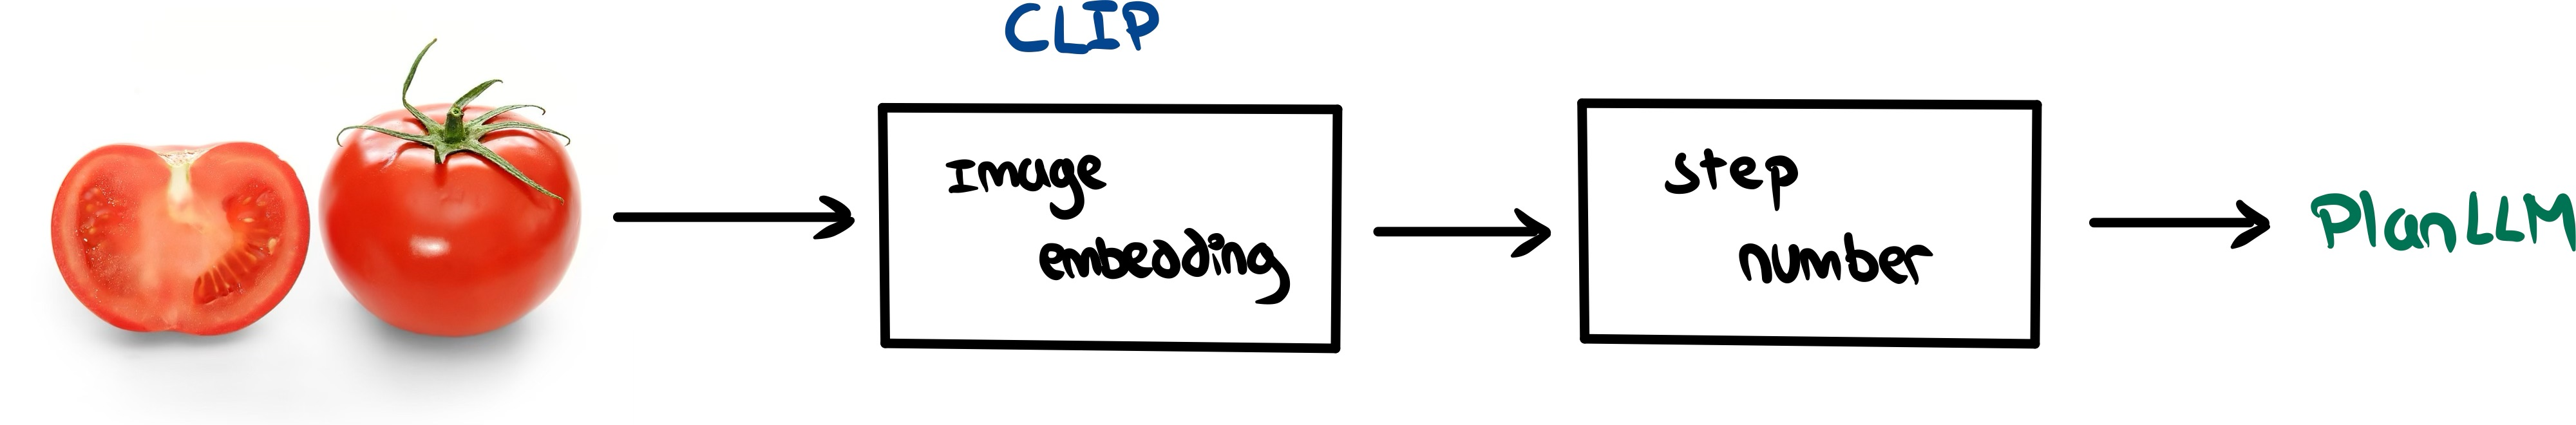
\includegraphics[scale=0.08]{images/planLLM.jpg}
    \caption{Image passing to PlanLLM}
\end{figure}

In order to re-create a conversation like the one above we need to carefully manipulate the JSON to get the answers we want. We detected that the PlanLLM isn't very good at jumping from steps (for instance if the user wants to begin with step 5 instead of 1). But the model is very responsive when the user says exactly \textbf{"I am currently on step x"} and the PlanLLM updates it's current step variable to the one given by the user.

Since we want a more fluid and natural conversation because the user's isn't supposed to always say the exact phrase \textbf{"I am currently on step x"}. For that we allow the user to either send a text or an image and we predict what is the step in the recipe that the users refers to by comparing the embedding scores and finding our which of is the best one. With this mechanism that we developed with the help of CLIP we allow the user to jump between steps as much as they like. Now what is left is the whole orchestration of the dialog with the user and that we will cover in the next chapter.

\subsection{Contextual Embedding and Self-Attention Analysis}
\subsubsection{Contextual Embeddings:}
Let's analyse the contextual embedding of two phrases and look at the evolution in layers.

\begin{figure}[!htbp]
    \center
    \includegraphics[scale=0.2]{images/contextual\_embeddings}
    \caption{Contextual embeddings over layers}
\end{figure}
We can see that with the evolution of the layers the tokens that are indeed related to each other are in a cluster different from the other tokens. At deeper layers, the model can capture increasingly abstract and complex semantic relationships between words and phrases. This allows it to form more precise clusters based on deeper semantic meaning rather than just surface-level similarities. Also as we progress through the layers the model has more contextual information to work with.
\subsubsection{Positional Embeddings:}
In here let's analyse a simple BERT encoder and we will work with a sequence text with the same word repeated 20 times.\\[10pt]

\begin{figure}[!htbp]
    \center
    \includegraphics[scale=0.3]{images/positional\_embeddings}
    \caption{Positional embeddings of a text with the same word}
\end{figure}

In here we can observe that in the diagonal we have a similarity of 1 and it makes sense we are comparing the same position with itself. But there is a strange behaviour in the first column and row. Between the first position and the second one we have a lower similarity score compared to the first and last one. That phenomena might be explained by the fact the both the first and last word only have one neighbour and therefore they are "similar". 
\subsubsection{Self Attention:} 
Here we will explore the difference of \textbf{cross encoder} and \textbf{dual encoder}. By passing the same two phrases to both these types of encodings we will get different results and let's explore why is that.\\[5pt]

\hspace{0.5cm} % Adjust the value as needed for the desired horizontal shift
\begin{minipage}{1.2\textwidth} % Adjust width as needed
\begin{dialogue}
\speak{Text1} "How to make pasta?"
\speak{Text2} "How much 1KG of pasta costs?"\\[5pt]
\end{dialogue}
\end{minipage}
By performing a dual encoding we encode one phrase and then the second one and then we calculate the similarity score. If we use~\cite{reimers-2019-sentence-bert} encoder with these two phrases we will get an approximate score of 0.72. Both the phrases are talking about pasta but in very different contexts. If we perform a cross encoding with the same model we will encode both phrases in the same context therefore the embeddings that will be calculated will have in mind the context of both the phrases and we will get a much better result (a lower score) but it makes sense since the phrases are talking about two different things eventhough they mention pasta in it.
\section{Evaluation}
\subsection{Dataset Description}
The dataset contains a significant amount of recipe information, but not all of it is pertinent to our objectives. After careful examination, we have identified the essential data required for generating meaningful embeddings and providing accurate search results to users. Our focus has been on excluding irrelevant information and prioritizing specific details that enhance the user's search experience.

Following a thorough dataset analysis, we selectively filtered the essential data required for crafting our embeddings and information pertinent to users for search results. Our assessment highlighted the necessity for detailed information on certain aspects while deeming others less crucial.

During our process of embedding sentences and experimenting with various techniques, we encountered two significant problems. Firstly, the \textbf{displayText} of each ingredient contained excessive information, including opinions and irrelevant text. Secondly, some \textbf{displayText} entries were in languages other than English (e.g., Italian). This posed challenges, as searching for ingredients like Italian cheese would erroneously suggest a strong relationship due to language inconsistencies.

Therefore, to address these issues, we implemented two solutions. Firstly, we opted to utilize only the \textbf{ingredient} property of each ingredient. To accomplish this, we employed a model that extracts the ingredient from the \textbf{displayText} and populates the ingredient field in the JSON.

For that, we used the \url{https://github.com/strangetom/ingredient-parser}~\cite{ingredientParser} in order to extract the ingredients from a phrase. With this we solved the issue of having \textbf{null} values in these fields. However, the problem persisted with \textbf{textDisplay} being in another language, as the ingredient parser model~\cite{ingredientParser} simply returned the \textbf{displayText} as it was originally.

By utilizing a translator model~\cite{deeptranslate} before feeding the data to the ingredient parser~\cite{ingredientParser}, we successfully translated the \textbf{displayTexts} that were in other languages into English. This allowed us to apply the model to extract the ingredients and populate the missing fields.

These modifications to our original dataset resulted in a more comprehensive dataset. We created a new JSON file containing all of the original information along with the additional data. This file is accessible through OpenSearch, as it is stored without being indexed. Its sole purpose is to be retrievable from OpenSearch.

\subsection{PlanLLM Description}
Each step now has an embedding that was encoded with CLIP and we store all of those embeddings locally. Some steps have an image associated with them and we also store the embedding of that image on our local file. Every time we work in the context of a recipe we access this file in order get similarities that we want by doing the inner product to calculate the similarity score with CLIP ~\cite{clip} . We decided to do this locally since it didn't make much sense to put this extra overhead into OpenSearch.

While doing the conversation with PlanLLM when we get a response from the API we update our JSON that communicates with the PlanLLM in order to use it in the next conversation.
\bibliographystyle{plain}
\bibliography{my_bib}

\end{document}
